\documentclass[tikz]{standalone}
\usepackage{tikz}
\usepackage{amsmath}
\usepackage{xcolor}

\usetikzlibrary{calc}

\begin{document}
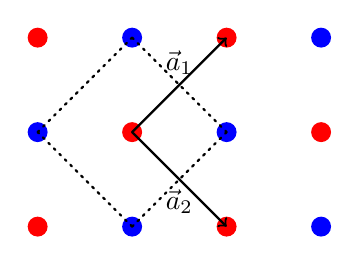
\begin{tikzpicture}[scale=1.2]

\def\N{3}
\def\M{2}
\def\d{1}

\foreach \i in {0,...,\N} {
  \foreach \j in {0,...,\M} {
    \pgfmathtruncatemacro{\isEven}{mod(\i+\j,2)}
    \ifnum\isEven=0
      \fill[red] (\i*\d, \j*\d) circle (3pt);
    \else
      \fill[blue] (\i*\d, \j*\d) circle (3pt);
    \fi
  }
}

\coordinate (O) at (0, \d);
\coordinate (A1) at ($(O) + (\d, \d)$);
\coordinate (A2) at ($(O) + (\d, -\d)$);
\coordinate (C) at ($(O) + (2*\d, 0)$);

\draw[thick, dotted, cap=round] (O) -- (A1);
\draw[thick, dotted, cap=round] (A1) -- (C);
\draw[thick, dotted, cap=round] (C) -- (A2);
\draw[thick, dotted, cap=round] (A2) -- (O);

\draw[->, thick, cap=round] ($(O) + (\d, 0)$) -- ($(O) + (2*\d,  \d)$) node[midway, above] {$\vec{a}_1$};
\draw[->, thick, cap=round] ($(O) + (\d, 0)$) -- ($(O) + (2*\d, -\d)$) node[midway, below] {$\vec{a}_2$};

\end{tikzpicture}
\end{document}
